\section{Durchführung}
\label{sec:Durchführung}
In der Durchführung des Versuchs wird zuerst eine Schaltung aufgebaut mit deren Hilfe die generelle Funktionsweise eines Lock-In-Verstärkers untersucht wird. Im zweiten Versuchsteil wird eine Photodetektorschaltung aufgebaut, mit der die Lichtintensität einer LED in Abhängigkeit des Abstandes zwischen  der LED und der genutzten Photodiode untersucht wird.
\subsection{Untersuchung der Funktionsweise eines Lock-In-Verstärkers}
Der schmatische Aufbau der genutzten Schaltung für die Untersuchung der Funktionsweise eines Lock-In-Verstärkers ist in \autoref{fig:schema2} dargestellt.
\begin{figure}[H]
    \centering
    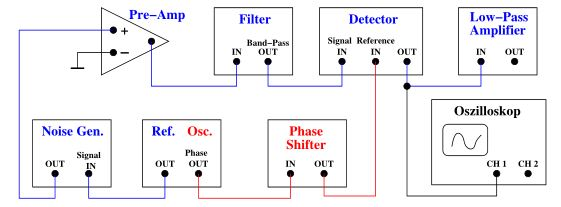
\includegraphics{images/schema2.JPG}
    \caption{Schematischer Aufbau der Messschaltung zur Untersuchung der Funktionsweise eines Lock-In-Verstärkers. \cite{sample}}
    \label{fig:schema2}
\end{figure}
\noindent
Zur praktischen Realisierung der Schaltung aus \autoref{fig:schema2} wird die Apparatur aus \autoref{fig:app} genutzt. Dazu werden die Anschlüsse entsprechend \autoref{fig:schema2} verschaltet.
\begin{figure}[H]
    \centering
    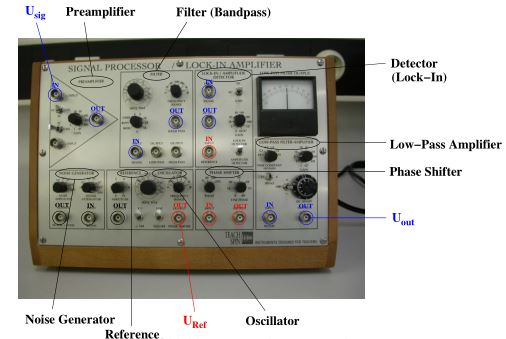
\includegraphics{images/schaltung.JPG}
    \caption{Schaltapparatur für die Realisierung eines Lock-In-Verstärkers. \cite{sample}}
    \label{fig:app}
\end{figure}
\noindent
Im ersten Teil der Messung wird der Noise Generator nicht genutzt, damit die Abhängigkeit zwischen der Phase der Referenzspannung und der Ausgangsspannung untersucht werden kann. Dabei werden sieben Messwerte zu der Phase der Referenzspannung und der Ausgangsspannung notiert. \newline
Im Anschluss wird der Noise-Generator angeschaltet, um den Einfluss eines zusätzlichen Rauschens auf die Spannung zu untersuchen. Dazu wird auf dem Oszilloskop ein Bild der Spannung mit eingeschaltetem Noise-Generator und ein Bild ohne Noise-Generator aufgenommen. 
\subsection{Photodetektorschaltung}
Für die Untersuchung der Lichtintensität der genutzten LED wird eine Photodetektorschaltung nach \autoref{fig:photo} aufgebaut.
\begin{figure}[H]
    \centering
    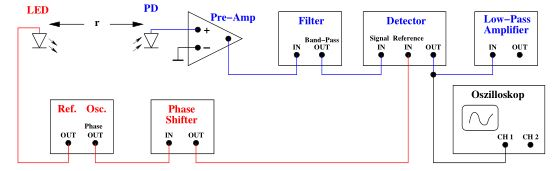
\includegraphics{images/photo.JPG}
    \caption{Schematischer Aufbau der Photodetektorschaltung zur Untersuchung der Lichtintensität der LED. \cite{sample}}
    \label{fig:photo}
\end{figure}
\noindent
Bei dieser Schaltung wird dann der Abstand zwischen LED und Photodiode nach und nach variiert und dabei werden Messwerte von dem Abstand zwischen LED und Photodiode sowie der gemessenen Spannung notiert.